\documentclass[11pt]{article}
\usepackage[margin=1in]{geometry}
\usepackage[T1]{fontenc}
\usepackage{lmodern}
\usepackage{amsmath,amssymb}
\usepackage{booktabs}
\usepackage{graphicx}
\usepackage{xcolor}
\usepackage[numbers,sort&compress]{natbib}
\usepackage[colorlinks=true,linkcolor=blue!50!black,citecolor=blue!50!black,urlcolor=blue!50!black]{hyperref}
\usepackage{caption}
\captionsetup{font=small,labelfont=bf}

\title{Topology-Aware Line Simplification for Web Maps:\\A Pixel-Tolerance Benchmark on Natural Earth}
\author{Kaisi Omar\\[2pt]
\small Aberystwyth University, United Kingdom\\
\small\url{https://github.com/sidewalkds-oss/geosimplify}}
\date{October 2026}

\begin{document}
\maketitle

\begin{abstract}
Web maps simplify borders and coastlines for each zoom level, typically with a
tolerance of about one pixel. When countries are simplified one at a time, the
two copies of each shared border diverge, opening gaps and overlaps and making
boundaries cross. We measure these effects on Natural Earth 1:10m countries
(548k vertices) and coastline at zoom levels 2--8. We compare radial distance,
Douglas--Peucker and Visvalingam--Whyatt in three modes: independent, shared
arcs, and shared arcs with a Saalfeld-style repair of crossings and side
changes. We also compare against the GEOS coverage simplifier. At zoom 4,
independent Douglas--Peucker opens 857 sliver gaps, creates 786 square pixels of
overlap, and makes 67 countries invalid. Shared arcs remove nearly all overlap
but leave 878 crossings and 62 invalid countries. Repair removes every crossing,
gap and invalid country at zoom 4 for 2.2\% more vertices and 1.5\% more
vector-tile geometry bytes. At an equal budget of 10\% of vertices, Douglas--Peucker has 4--8 times
smaller displacement than the alternatives, while Visvalingam--Whyatt best
preserves area but can move individual vertices tens of kilometres. The GEOS
coverage simplifier produced no invalid geometry at any zoom and ran 4--17 times
faster. Repaired Douglas--Peucker produced 15--27\% smaller geometry payloads at
zooms 4--8, with one-pixel-bounded displacement. Code, data scripts and results
are released as \texttt{geosimplify}.
\end{abstract}

%=====================================================================
\section{Introduction}

Every web map that draws country borders or coastlines at small scales
simplifies them first. At zoom level 2 a pixel covers almost 40\,km, and drawing
the half-million vertices of a 1:10m world map would waste bandwidth and
rendering time on detail no one can see. Vector-tile pipelines therefore
simplify geometry for each zoom level, typically with a tolerance of about one
pixel or one tile unit~\citep{tippecanoe,mvt21}.

The algorithms are old and well understood. Douglas--Peucker~\citep{ramer1972,douglas1973}
bounds the distance between the original and the simplified line.
Visvalingam--Whyatt~\citep{visvalingam1993} removes vertices in order of the
area they contribute and tends to preserve shape and area. Radial distance
filtering drops vertices that are too close together. Their trade-offs have
been evaluated many times~\citep{mcmaster1986,visvalingam1990,visvalingam1995,shi2006,song2016}.

Less often measured is what simplification does to a \emph{coverage}: a set of
polygons that tile the land without gaps or overlaps, such as countries. When
each polygon is simplified on its own, the two copies of a shared border are
simplified differently. Thin \emph{gaps} open between neighbours, and
\emph{overlaps} appear where both claim the same land. Simplification can also
make a boundary cross itself or a neighbour. Production tools address this by
simplifying shared borders once~\citep{topojson,harrower2006,tippecanoe} or with
coverage-aware simplifiers~\citep{jtscoverage}, and the computational-geometry
literature offers topology-preserving algorithms~\citep{deberg1998,saalfeld1999,estkowski2001,corcoran2011}.
We found no benchmark, however, that quantifies these errors on a real global
coverage at web-map zoom levels, or reports what preventing them costs in
vertices and vector-tile bytes.

\paragraph{Contributions.}
We provide a reproducible, web-map-oriented empirical comparison:
\begin{enumerate}
\item Three algorithms (radial distance, Douglas--Peucker,
  Visvalingam--Whyatt), each run in three modes: independent per ring, shared
  arcs (TopoJSON-style), and shared arcs with a Saalfeld-style crossing repair.
  We also compare against the GEOS coverage simplifier.
\item Measurements at zoom levels 2--8 with a one-pixel tolerance on Natural
  Earth 1:10m countries and coastline: vertex retention, displacement in
  screen pixels, area change, invalid geometries, segment crossings, sliver
  gaps and overlaps between neighbours, and Mapbox Vector Tile geometry bytes.
\item An efficient implementation, \texttt{geosimplify}. It precomputes each
  vertex's significance once, so any zoom level becomes a threshold, and it
  ships with the benchmark and a test suite that checks it against textbook
  implementations.
\end{enumerate}

%=====================================================================
\section{Related work}

\paragraph{Line simplification.}
The Ramer--Douglas--Peucker algorithm~\citep{ramer1972,douglas1973} recursively
keeps the vertex farthest from the current chord while that distance exceeds a
tolerance, so every removed vertex lies within the tolerance of the result.
Visvalingam and Whyatt~\citep{visvalingam1993} instead repeatedly eliminate the
vertex whose triangle with its neighbours has the smallest area. Visvalingam and
Whyatt also critiqued Douglas--Peucker through
visualisation~\citep{visvalingam1990}, and Visvalingam and Williamson compared
the two on road data~\citep{visvalingam1995}. McMaster~\citep{mcmaster1986}
analysed geometric measures of simplification quality. Shi and
Cheung~\citep{shi2006} evaluated algorithms for vector generalisation, and Song
and Miao~\citep{song2016} proposed an evaluation aimed at map visualisation.
Kronenfeld et al.~\citep{kronenfeld2020} simplify by segment collapse to
minimise areal displacement.

\paragraph{Topological consistency.}
Saalfeld~\citep{saalfeld1999} made Douglas--Peucker topologically consistent
by detecting conflicts and refining the simplification where they occur. de
Berg, van Kreveld and Schirra~\citep{deberg1998} simplify whole subdivisions
without changing their topology. Estkowski and
Mitchell~\citep{estkowski2001} studied the complexity of keeping a simplified
subdivision simple, and Wu and M\'arquez~\citep{wu2003} proposed a
non-self-intersecting Douglas--Peucker. Corcoran et al.~\citep{corcoran2011}
addressed planar and non-planar consistency for vector maps, Mustafa et
al.~\citep{mustafa2006} simplified large maps dynamically for visualisation,
and Gruppi et al.~\citep{gruppi2015} gave a topologically correct
Visvalingam--Whyatt heuristic. Our repair mode follows Saalfeld's idea and is not
a new algorithm.

\paragraph{Tools.}
TopoJSON~\citep{topojson} and mapshaper~\citep{harrower2006} split polygon
boundaries into shared arcs so that neighbours are simplified identically.
tippecanoe~\citep{tippecanoe} simplifies per zoom level when building vector
tiles. JTS and GEOS provide a coverage simplifier based on
Visvalingam--Whyatt~\citep{jtscoverage}, which we use as a baseline through
Shapely~\citep{shapely}.

%=====================================================================
\section{Method}
\label{sec:method}

\paragraph{Projection and tolerance.}
Geometries are projected to Web Mercator, the projection of web-map tiles. At
zoom $z$ a 256-pixel tile spans $2\pi R/2^z$ metres, so a screen pixel is
$r_z = 2\pi R/(256\cdot 2^z)$ metres at the equator ($R=6{,}378{,}137$\,m). We
simplify at a tolerance of one pixel, $\varepsilon = r_z$, and report distances
in pixels at the target zoom.

\paragraph{Algorithms as significance thresholds.}
For Douglas--Peucker we run the recursion once at zero tolerance and record,
for each vertex, the deviation at which it is inserted, capped by its
ancestor's value. Keeping the vertices whose significance exceeds
$\varepsilon$ then reproduces Douglas--Peucker at tolerance $\varepsilon$
exactly. For Visvalingam--Whyatt we record each vertex's \emph{effective area}:
the running maximum of the eliminated areas at the moment it is removed.
Keeping the vertices with effective area at least $\varepsilon^2$ reproduces
the algorithm at area threshold $\varepsilon^2$; GEOS uses the same
square-root-of-area convention. Our test suite checks both equivalences against
direct implementations at multiple tolerances. Every zoom level is then a cheap
threshold. Radial distance, which is not hierarchical, is run directly.

\paragraph{Modes.}
\emph{Independent}: every ring or line is simplified on its own, with its first
vertex fixed. \emph{Shared arcs}: we find \emph{junctions}, vertices whose
neighbouring vertices across all rings number more than two, and split every
ring there into arcs. Identical arcs, in either direction, are stored once and
simplified once with their endpoints fixed. A ring with no junction becomes a
closed arc starting at its lexicographically smallest vertex, so a shared ring
such as an enclave boundary gets the same arc from both sides. Each closed arc
also pins two more vertices that span a triangle, so it cannot collapse to a
line. \emph{Repair}: after shared-arc simplification, each round looks for two
kinds of conflict. \emph{Crossings}: we index every simplified segment of the
layer in an STR-tree and find pairs that cross or overlap; pairs that merely
share an endpoint are not counted. \emph{Side changes}: for every original
ring we take an interior point and record which other rings contain it. After
simplification, a ring that now contains a point it did not (or no longer
contains one it did) has changed side. This happens, for example, when a
straightened coastline swallows an offshore island without any segments
crossing. For each crossing segment, and for the segment of the offending ring
nearest each changed point, we restore the original vertex that deviates most
from that segment. Rounds repeat until no conflict remains or 30 rounds have
passed. The repair is local, adding one vertex per conflict instead of lowering
the tolerance of whole arcs, and it follows the conflict-and-refine idea of
Saalfeld~\citep{saalfeld1999}.

\paragraph{Metrics.}
\emph{Retention} is the share of vertices kept. \emph{Displacement} measures
each original vertex against the simplified segment that replaced it (between
the nearest kept vertices on either side). This is the error Douglas--Peucker
bounds, and it is never smaller than the discrete Hausdorff distance. We report
the 95th percentile, over features, of each feature's maximum displacement, in
pixels. \emph{Area change} is the total absolute change in country area divided
by the total area. \emph{Invalid features} are those that become invalid (for
polygons) or non-simple (for lines) although the original was not.
\emph{Crossings} counts simplified segments that cross another. \emph{Gaps} are
holes in the union of simplified countries that intersect no hole of the
original union: slivers of land that belong to no country. \emph{Overlap} is the
summed area of all countries minus the area of their union. Areas are reported
in square pixels. \emph{Bytes} is the size of the geometry command stream of
the Mapbox Vector Tile encoding~\citep{mvt21} on a 4096-unit-per-tile grid at
zoom $z$. It counts zig-zag delta-encoded coordinates and commands as varints,
and drops repeated grid points. We encode on the global grid without clipping
to tiles and omit feature and attribute overhead, so the figure measures the
geometry payload rather than a deployable tile size.

%=====================================================================
\section{Data and protocol}
\label{sec:data}

We use Natural Earth~\citep{naturalearth} 1:10m Admin-0 countries (258
features, 548{,}471 vertices) and 1:10m coastline (4{,}133 lines, 410{,}957
vertices), obtained from the project's GitHub repository. Countries form a
coverage with shared borders. Shared-arc decomposition reduces the 548k ring
vertices to 480k arc vertices, because about 68k vertices lie on borders shared
by two countries, and rebuilding from the unsimplified arcs reproduces every
country's area exactly. Two country features are already invalid in the source
and are excluded from the invalid-feature counts. We simplify for zoom levels
2, 4, 6 and 8 at one pixel. For the retention--error trade-off we sweep 13
tolerances from 100\,m to 100\,km in shared-arc mode. All runs are
deterministic. Timings are single-threaded Python on a consumer laptop and
indicate relative cost only.

%=====================================================================
\section{Results}
\label{sec:results}

\begin{figure}[t]
\centering
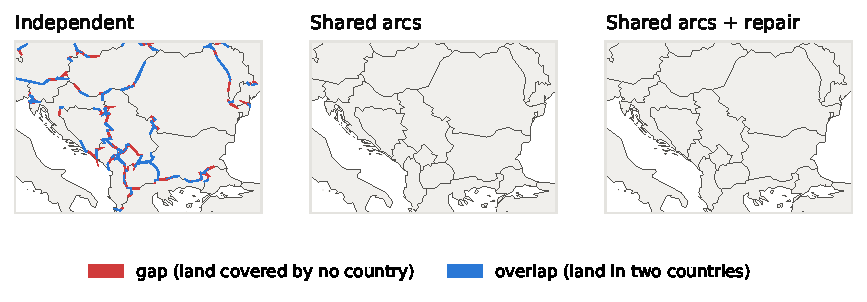
\includegraphics[width=\linewidth]{figures/fig1_example.pdf}
\caption{Douglas--Peucker simplification of the Balkans for zoom 4 (one-pixel
tolerance). Independent simplification opens gaps (red) and overlaps (blue)
along almost every border; shared arcs remove them.}
\label{fig:example}
\end{figure}

\paragraph{Independent simplification breaks the coverage.}
Figure~\ref{fig:example} shows the effect around the Balkans, and
Table~\ref{tab:countries} quantifies it worldwide at zoom 4. Simplifying each
country on its own with Douglas--Peucker opens 857 sliver gaps (1{,}201\,px$^2$),
creates 786\,px$^2$ of overlap, and makes 67 originally valid countries invalid,
with 2{,}452 crossing segments. Radial distance is worst. Its output depends on
where each ring starts, so the two copies of a border diverge almost
everywhere: 6{,}101 gaps and 16{,}970 crossings. Visvalingam--Whyatt is the
least affected (301 gaps) because its local, direction-independent elimination
often treats both copies of a border the same way. The problem persists at every
zoom level (Figure~\ref{fig:coverage}).

\begin{table}[t]
\centering\small
\caption{Countries (Natural Earth 1:10m) simplified for zoom 4 at one pixel
($r_4 = 9.8$\,km). Displacement is the 95th percentile over countries; KB is MVT
geometry payload; time is single-threaded Python.}
\label{tab:countries}
\resizebox{\linewidth}{!}{\begin{tabular}{llrrrrrrrr}
\toprule
Method & Mode & Retained & Disp.\ p95 (px) & Invalid & Crossings & Gaps & Overlap (px$^2$) & KB & Time (s) \\
\midrule
Radial distance & Independent & 27.5\% & 1.00 & 47 & 16970 & 6101 & 953.0 & 314 & 0.9 \\
 & Shared arcs & 27.6\% & 1.00 & 49 & 369 & 66 & 0.0 & 316 & 0.8 \\
 & Shared arcs + repair & 27.6\% & 1.00 & 0 & 31 & 0 & 0.0 & 316 & 35.8 \\
\midrule
Douglas–Peucker & Independent & 9.2\% & 1.00 & 67 & 2452 & 857 & 786.3 & 135 & 0.3 \\
 & Shared arcs & 9.1\% & 1.00 & 62 & 878 & 206 & 0.4 & 135 & 0.3 \\
 & Shared arcs + repair & 9.3\% & 1.02 & 0 & 0 & 0 & 0.0 & 137 & 15.9 \\
\midrule
Visvalingam–Whyatt & Independent & 12.3\% & 5.75 & 43 & 986 & 301 & 111.1 & 161 & 0.3 \\
 & Shared arcs & 12.3\% & 5.74 & 47 & 408 & 36 & 0.2 & 162 & 0.3 \\
 & Shared arcs + repair & 12.4\% & 5.64 & 0 & 0 & 0 & 0.0 & 163 & 14.9 \\
\bottomrule
\end{tabular}}
\end{table}

\paragraph{Shared arcs remove overlaps but not crossings.}
Simplifying each border once removes divergence. Overlap falls by three orders
of magnitude, to at most 0.35\,px$^2$ at zoom 4, and gaps fall by 3 to over
1{,}000 times depending on algorithm and zoom, with essentially no change in
vertex count or bytes. But shared arcs do not stop a simplified
border from crossing a neighbouring arc or swallowing an island. With
Douglas--Peucker at zoom 4, 878 crossings, 31 ring-side conflicts and 62 invalid
countries remain, and the 206 remaining gaps are their by-products.

\paragraph{Repair removes the rest at little cost.}
With the repair, Douglas--Peucker and Visvalingam--Whyatt reach zero crossings,
zero side conflicts, zero gaps, zero overlap and zero invalid countries at zoom
4. The price is small (Table~\ref{tab:repair}). Douglas--Peucker keeps 2.2\%
more vertices at zoom 4 (1{,}088 restored vertices) and its geometry payload
grows by 1.5\%; at zoom 8 the overhead is 45 vertices. The 95th-percentile
displacement can rise slightly above one pixel (1.02--1.05\,px at zooms 2--4),
because a restored vertex tilts the segments around it. Repair is the slowest
step, taking 15--36\,s per layer and zoom in our pure-Python implementation,
since each round re-indexes every segment. Without repair a zoom level takes
about 1\,s once vertex significance is cached; computing it is a one-time cost
of about 10\,s per layer for Douglas--Peucker.

\begin{table}[t]
\centering\small
\caption{Cost of the repair relative to shared arcs alone: extra vertices
(\%) / restored vertices, per zoom level (countries).}
\label{tab:repair}
\begin{tabular}{lcccc}
\toprule
Method & z2 & z4 & z6 & z8 \\
\midrule
Radial distance & +2.0\% / 993 & +0.3\% / 393 & +0.0\% / 72 & +0.0\% / 2 \\
Douglas–Peucker & +8.4\% / 1785 & +2.2\% / 1088 & +0.3\% / 416 & +0.0\% / 45 \\
Visvalingam–Whyatt & +5.6\% / 1310 & +0.8\% / 521 & +0.0\% / 93 & +0.0\% / 3 \\
\bottomrule
\end{tabular}
\end{table}

\begin{figure}[t]
\centering
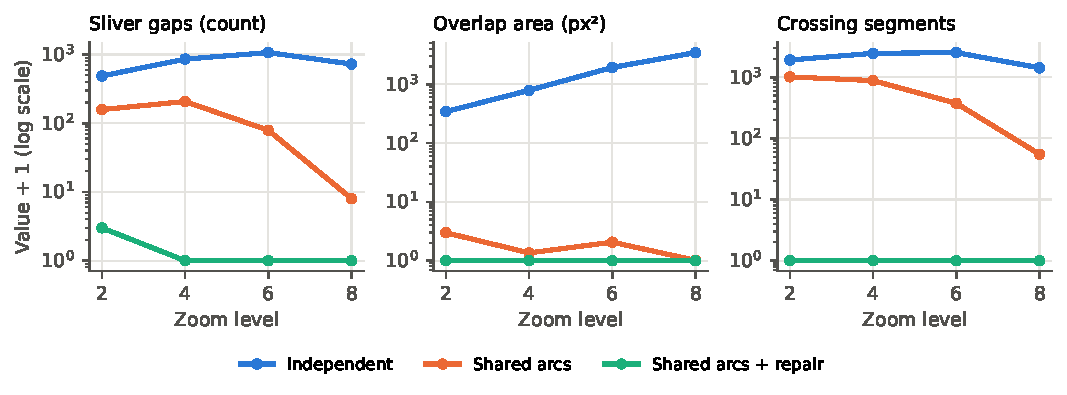
\includegraphics[width=\linewidth]{figures/fig3_coverage_errors.pdf}
\caption{Coverage errors of Douglas--Peucker by zoom level and mode
(countries). Values are shifted by one for the logarithmic axis.}
\label{fig:coverage}
\end{figure}

\paragraph{What remains.}
At zoom 2, where a pixel is 39\,km, two countries remain invalid after repair
with Douglas--Peucker and three with Visvalingam--Whyatt. Each corresponds to a
side conflict that the repair could not resolve within 30 rounds. Radial
distance keeps 31 crossings at every zoom level. These are present in the
source data: Natural Earth 1:10m contains 31 pairs of crossing segments at full
resolution, which no vertex restoration can remove. At zooms 6 and 8 one or two
countries remain invalid with no detected conflicts, a defect class our checks
do not cover (for example a ring touching itself at a single point). Between
eight and nine small countries vanish at zoom 2 in shared-arc modes: their
boundaries consist of several arcs that each shrink to their endpoints. This is
sub-pixel detail, but a renderer that must show every country would need a
minimum-size rule.

\paragraph{Coastlines.}
The coastline layer has no shared borders, but the same crossing problem
appears (Table~\ref{tab:coast}). Independent Douglas--Peucker at zoom 4 creates
896 crossings and 71 self-intersecting lines. Repair removes them all for 1.7\%
more vertices.

\begin{table}[t]
\centering\small
\caption{Coastline (Natural Earth 1:10m) simplified for zoom 4 at one pixel.}
\label{tab:coast}
\resizebox{\linewidth}{!}{\begin{tabular}{llrrrrrr}
\toprule
Method & Mode & Retained & Disp.\ p95 (px) & Invalid & Crossings & KB & Time (s) \\
\midrule
Radial distance & Independent & 28.0\% & 0.87 & 68 & 350 & 252 & 0.4 \\
 & Shared arcs + repair & 28.2\% & 0.86 & 0 & 12 & 253 & 27.6 \\
\midrule
Douglas–Peucker & Independent & 11.1\% & 0.98 & 71 & 896 & 127 & 0.0 \\
 & Shared arcs + repair & 11.3\% & 0.98 & 0 & 0 & 129 & 10.7 \\
\midrule
Visvalingam–Whyatt & Independent & 13.8\% & 1.47 & 23 & 349 & 144 & 0.0 \\
 & Shared arcs + repair & 13.9\% & 1.34 & 0 & 0 & 145 & 9.7 \\
\bottomrule
\end{tabular}}
\end{table}

\paragraph{Algorithms at equal vertex budgets.}
At a fixed tolerance the three algorithms keep very different numbers of
vertices: 9\%, 12\% and 28\% for Douglas--Peucker, Visvalingam--Whyatt and
radial distance at zoom 4. We therefore compare them along their trade-off
curves (Figure~\ref{fig:pareto}, Table~\ref{tab:budget}). For the same number
of vertices, Douglas--Peucker has by far the smallest displacement: at 10\% of
vertices its 95th-percentile displacement is 8.6\,km, against 34\,km for radial
distance and 69\,km for Visvalingam--Whyatt. Visvalingam--Whyatt preserves area
best: 0.034\% total area change at 10\%, against 0.088\% for Douglas--Peucker
and 0.12\% for radial distance. These are the expected strengths of a
distance-bounded and an area-driven method. The size of the gap at real scale is
notable, however. Visvalingam--Whyatt's displacement is unbounded: in our sweep
a single vertex moved 53\,km even at a 100\,m tolerance, because the algorithm
removes long, thin features such as spits and fjords whose triangles have small
area.

\begin{figure}[t]
\centering
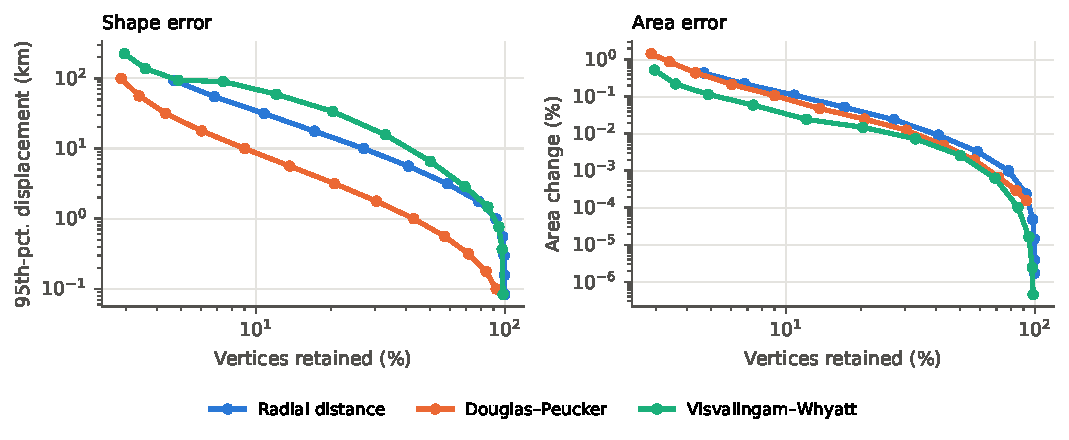
\includegraphics[width=\linewidth]{figures/fig2_pareto.pdf}
\caption{Trade-off between vertices retained and error (countries, shared
arcs, 13 tolerances from 100\,m to 100\,km).}
\label{fig:pareto}
\end{figure}

\begin{table}[t]
\centering\small
\caption{Displacement (95th percentile) / total area change at equal vertex
budgets, interpolated along the curves of Figure~\ref{fig:pareto}.}
\label{tab:budget}
\begin{tabular}{lccc}
\toprule
Method & 5\% of vertices & 10\% of vertices & 25\% of vertices \\
\midrule
Radial distance & 84.8 km / 0.39\% & 34.4 km / 0.12\% & 11.0 km / 0.03\% \\
Douglas–Peucker & 24.7 km / 0.33\% & 8.6 km / 0.09\% & 2.4 km / 0.02\% \\
Visvalingam–Whyatt & 93.5 km / 0.11\% & 69.4 km / 0.03\% & 24.3 km / 0.01\% \\
\bottomrule
\end{tabular}
\end{table}

\paragraph{Bytes.}
Figure~\ref{fig:bytes} relates simplification to vector-tile payload. With
repair, Douglas--Peucker reduces the geometry payload to 6.9\% of the
unsimplified (grid-snapped) encoding at zoom 2, 12.7\% at zoom 4, 33.6\% at
zoom 6 and 67.2\% at zoom 8. Visvalingam--Whyatt needs 7.1\%, 15.1\%, 46.2\% and
88.8\%, and radial distance 12.5\%, 29.4\%, 69.8\% and 98.2\%. Bytes track
retained vertices closely. At one pixel, Douglas--Peucker gives the smallest
tiles, and preventing gaps, overlaps and crossings costs at most a few percent.

\begin{figure}[t]
\centering
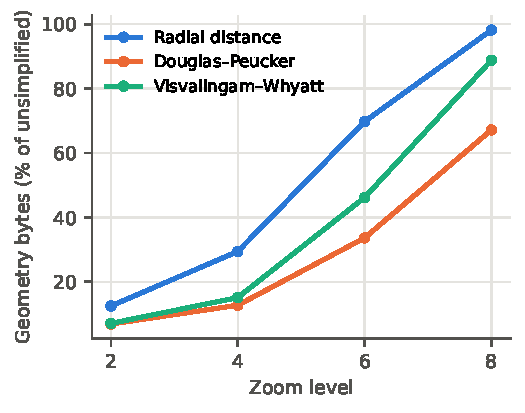
\includegraphics[width=0.55\linewidth]{figures/fig4_bytes.pdf}
\caption{MVT geometry payload after simplification with repair, relative to
the unsimplified layer encoded on the same grid.}
\label{fig:bytes}
\end{figure}

%=====================================================================
\section{Comparison with GEOS coverage simplification}
\label{sec:baseline}

GEOS, through Shapely~\citep{shapely}, provides a coverage simplifier ported
from JTS~\citep{jtscoverage}. It is based on Visvalingam--Whyatt, preserves
coverage topology, and uses the same square-root-of-area tolerance as our
Visvalingam--Whyatt. Table~\ref{tab:baseline} compares it with our two repaired
modes at the same one-pixel tolerances. Because it does not report which
vertices it kept, all three are scored by GEOS's discrete Hausdorff distance
rather than our displacement.

\begin{table}[t]
\centering\small
\caption{GEOS CoverageSimplifier against shared arcs + repair (countries,
one-pixel tolerance). Hausdorff distances are discrete, in pixels at the
target zoom; \emph{Dropped} counts countries that vanish entirely.}
\label{tab:baseline}
\resizebox{\linewidth}{!}{\begin{tabular}{llrrrrrrrr}
\toprule
Zoom & Method & Vertices & Hausd.\ p95 (px) & Hausd.\ max (px) & Invalid & Dropped & Gaps & KB & Time (s) \\
\midrule
z2 & GEOS CoverageSimplifier & 23.6k & 2.26 & 7.9 & 0 & 0 & 0 & 61 & 3.9 \\
 & Douglas--Peucker + repair & 23.2k & 1.00 & 2.7 & 2 & 9 & 2 & 62 & 36.1 \\
 & Visvalingam--Whyatt + repair & 24.8k & 2.28 & 7.9 & 3 & 8 & 3 & 63 & 24.8 \\
\midrule
z4 & GEOS CoverageSimplifier & 66.8k & 4.95 & 13.7 & 0 & 0 & 0 & 160 & 3.6 \\
 & Douglas--Peucker + repair & 50.8k & 1.00 & 6.3 & 0 & 5 & 0 & 137 & 16.1 \\
 & Visvalingam--Whyatt + repair & 67.6k & 4.89 & 8.0 & 0 & 5 & 0 & 163 & 15.0 \\
\midrule
z6 & GEOS CoverageSimplifier & 218.7k & 3.82 & 54.9 & 0 & 0 & 0 & 521 & 2.4 \\
 & Douglas--Peucker + repair & 134.7k & 1.00 & 1.4 & 1 & 0 & 0 & 381 & 27.6 \\
 & Visvalingam--Whyatt + repair & 219.5k & 3.68 & 6.1 & 0 & 1 & 0 & 523 & 24.7 \\
\midrule
z8 & GEOS CoverageSimplifier & 453.4k & 2.73 & 219.4 & 0 & 0 & 0 & 1258 & 2.1 \\
 & Douglas--Peucker + repair & 299.8k & 1.00 & 1.0 & 2 & 0 & 0 & 952 & 21.4 \\
 & Visvalingam--Whyatt + repair & 453.7k & 2.22 & 7.5 & 0 & 0 & 0 & 1259 & 34.6 \\
\bottomrule
\end{tabular}}
\end{table}

The GEOS simplifier is the most robust. It produced no invalid countries, no
gaps and no dropped countries at any zoom, in 2--4\,s per layer, 4 to 17 times
faster than our repair. Its vertex counts and bytes are almost identical to our
repaired Visvalingam--Whyatt, as expected from the shared algorithm and
tolerance convention. Repaired Douglas--Peucker is the most compact. At zooms
4--8 it keeps 24--38\% fewer vertices than GEOS and its geometry payload is
15--27\% smaller. Its 95th-percentile Hausdorff distance stays at one pixel,
against 2.3--5.0\,px for GEOS, but one or two countries remain invalid at zooms
2, 6 and 8. The area-driven simplifiers also have rare large outliers: GEOS's
maximum Hausdorff distance reaches 55\,px at zoom 6 and 219\,px at zoom 8,
against at most 6.3\,px for repaired Douglas--Peucker.

In practice, the GEOS coverage simplifier is the safer default for producing
valid coverages. A distance-bounded simplifier with repair produces smaller
tiles and tighter shape fidelity, at the cost of slower processing and a small
residue of invalid geometry that would need a final validity pass.

%=====================================================================
\section{Discussion and limitations}

\paragraph{Recommendations for tile pipelines.}
(1) Never simplify neighbouring polygons independently: at a one-pixel
tolerance this opened tens to thousands of sliver gaps worldwide at every
zoom level. (2) Shared arcs are necessary but not sufficient. Crossings and
swallowed islands also need a repair step or a coverage-aware simplifier.
(3) Use Douglas--Peucker when bytes and bounded displacement matter most, and an
area-based method when area and visual smoothness matter more, keeping in mind
that area-based methods can move individual vertices tens of pixels.
(4) Check validity after simplification. Even the repaired outputs left one to
three invalid countries at some zoom levels, and the source data itself
contains crossing segments.

\paragraph{Limitations.}
We evaluate one global dataset at one scale (1:10m) and one pixel tolerance;
other data, such as dense administrative subdivisions or road networks, may
behave differently. Byte counts measure the MVT geometry command stream on the
global grid without tile clipping, buffers, attributes or compression, so they
show relative rather than absolute tile sizes. Our displacement measure respects
vertex order and bounds the discrete Hausdorff distance, but neither captures
perceived shape quality. Our implementation is pure Python, so its timings are
not comparable with GEOS's C++ in absolute terms, and the repair's round-based
re-indexing could be made incremental. Our side-change test uses one interior
point per ring and can miss conflicts that do not move that point, and we did
not attempt to repair rings that touch themselves at a single point.

%=====================================================================
\section{Conclusion}

On a real global coverage, independent simplification at web-map tolerances
reliably breaks the map. It opens tens to thousands of slivers between
countries, creates overlaps, and makes dozens of countries invalid. Simplifying
shared borders once removes the overlaps, and a Saalfeld-style repair of
crossings and side changes removes nearly all remaining defects for about 2\%
more vertices. The GEOS coverage simplifier achieves complete validity faster;
repaired Douglas--Peucker yields smaller tiles with one-pixel-bounded
displacement. All code, data-download scripts and results are available for
reproduction.

\paragraph{Reproducibility.}
\texttt{python experiments/download\_data.py} fetches the data;
\texttt{run\_benchmark.py} and \texttt{run\_coverage\_baseline.py} regenerate
every CSV in \texttt{results/}; and \texttt{make\_figures.py} regenerates every
figure and table.

\bibliographystyle{plainnat}
\bibliography{references}

\end{document}
